% Chapter Template
\chapter{Monitoring Tool - Implementation and Deployment} % Main chapter title

\label{Chapter4} % Change X to a consecutive number; for referencing this chapter elsewhere, use \ref{ChapterX}

\lhead{Chapter 4. \emph{Monitoring Tool - Part 2}} 

\section{NetwObserver}
The first step in the development was to select the technologies adapted to the problem. As we had a lot of log to parse, we have started the implementation using Python. Python has a strong integration of the strings and lists. It's quite easy to generate a parser of logs and keeping the code neat thanks to its very simple syntax.
As more feature were added, we need to structure the system in a way that make it easily accessible. It's a monitoring tools and it has to be accessible from everywhere and easy to use. So, we decided to implemented it as a web application. This application would be usable from every computer without any installation and the network administrators could manage and maintain it directly on the server. An update would be accessible directly for every users.

\subsection{Django: A High-Level Python Web Framework}
As presented by its developers, Django is a "web framework for perfectionist with deadlines"\footnote{\url{https://www.djangoproject.com/}}. Django allow to achieve a modular structure quite easily and provide all the developers need to add new components in the application. A Django application is composed of several modules that exists independently and interact with each other through the database.
Moreover, Django adhere to the DRY\footnote{\url{http://c2.com/cgi/wiki?DontRepeatYourself}} principle.
\begin{description}
  \item[Don't Repeat Yourself] \hfill \\
  Every piece of knowledge must have a single, unambiguous, authoritative representation within a system.
\end{description}
When we use this framework, we focus on writing and defining each element one time on the right place. Maintainability is another important component of our system. Having duplication all over the code make it difficult to maintain and to keep coherent.
Django used a variation of the Model-View-Controller model called \emph{Model-View-Template}\cite{mvt}. The main difference is that Django is not about states. Browser don't evolve from one state to another, every request are done from scratch. In MVC, Controller update the View and the Model accordingly to the events. That's not the case here because each time something is modified (e.g a new insertion in the database) we start from the beginning. It's not a defect, it's how HTTP work.

\begin{description}
\item[Model] \hfill \\
The first element that composed the application are the entities manipulated by the application. A model is a representation of an element of the domain. Each model encapsulates all the data and information required to understand it.
\item[View] \hfill \\
The main task of the views is to handle the HTTP requests. It receives a HTTP request and returns a HTTP response.
\item[Template] \hfill \\
It represents the HTTP response. It provide a generic answer and the View fulfil the missing parts (most of the time by interrogating the database).
\end{description}

Like most of the modern web frameworks, Django is built using the \emph{Object-relational mapping} technique. The purpose is to make a bridge between the object manipulated by Python and the database entries. The architecture respects an \emph{Active-record pattern} that tied each object to a row in the database. It allow to focus on the logic of the application and to code easier. We can do more with less code. The main drawback of such pattern, it's that developers tend to forget the database behind it. Even if Django is optimised to translate object in database entity (and in the other way around), it important to design the model by thinking about the database hidden behind. Every access is translated by Django but poor request or weak design could lead to really poor performance.

\subsection{MySql}
Even if most of the time we don't make direct transaction with the database, it's important to chose the right DBMS\footnote{Database Management System}. At the beginning, the capacity of the application were quite limited and we used SqLite\footnote{\url{https://sqlite.org/}}. SqLite has the particularity to not use a client-server model. It is directly managed inside the application and it is the one used by default in Django. It fits really well to small applications because all actions are internally handled and it doesn't require to install an external DBMS to handle the transactions. But quickly, we reach the limits of SqLite and we chose to migrate to MySql. NetwObserver generates several threads and make a lot of concurrent accesses to the database. Such utilization is not adapted to SqLite and made the application unstable. The main issue was that, while the application is gathering its data, it needs to still be available to the users. SqLite have some difficulties to handle insertion of a lot of new entries while getting concurrent requests from the users.

\subsection{Gatherer}
The main difficulty was to correctly gather the source of information available. For each of them, we had to implement a module to make the interface between the sources and the database. They were quite heterogeneous and the implementation required a deep understanding of them.
\subsubsection{Logs Parser}
The first source we have processed were the log files. There are three generators of log file on the network: the controller, the DHCP and the Radius. Actually, there already is a software that gathers the log files and centralized them. The tool is called Octopussy\footnote{http://www.octopussy.pm/} and is a log management solution. It allows the administrators to display the log and access them by specifying criteria like date, source or the gravity of the log. Our \emph{log} module does basically the same thing but with a deeper analysis and understanding of the content of the logs. 
\paragraph{DHCP}
The DHCP generates a log for each step of the allocation of an IP address and of course when an error occurred. Typical logs look like this:
\begin{lstlisting}[frame=single,breaklines=true,caption={DHCP logs}]
2013-10-21T17:26:00.113154+02:00 dhcp-1 dhcpd: DHCPREQUEST for 192.168.32.43 from cc:fe:3c:26:5c:3f via 192.168.35.253
2013-10-21T17:26:00.113239+02:00 dhcp-1 dhcpd: DHCPACK on 192.168.32.43 to cc:fe:3c:26:5c:3f via 192.168.35.253
2013-10-21T17:26:00.196242+02:00 dhcp-1 dhcpd: DHCPDISCOVER from 50:a4:c8:6b:48:c7 via 130.104.175.250: load balance to peer dhcp1-dhcp2
\end{lstlisting}
When the application can understand each part of the message, it allows to make more powerful links between them. If we correctly analyse each messages, we can tell, for example, which \emph{dhcpAck} correspond to a \emph{dhcpRequest}. That's a weakness of Octopussy. It can tell you what log are important and filter them but it doesn't make analysis based on the protocol. DHCP defined a succession of actions and being able to trace them make the application capable of detecting more subtle errors. Concretely, the module \emph{log} decompose the message in several part and stock it in a relational database. Even if it could seem simple, having a structured representation of the log is the first step to make better analysis on them.

\paragraph{Radius}
Radius generates logs about the authentication of the users. The main information here is the \emph{login} entered and the device used for the authentication.
\begin{lstlisting}[frame=single,breaklines=true,caption={Radius logs}]
2013-10-21T17:26:00+02:00 radius1.sri.ucl.ac.be radiusd[1523]: [ID 702911 local3.notice] Login OK: [@eur.nl] (from client WiSMPythagore-B port 29 cli e4-d5-3d-89-af-51)
2013-10-21T17:26:05+02:00 radius1.sri.ucl.ac.be radiusd[17913]: [ID 702911 local4.notice] Login incorrect: [none] (from client WiSMPythagore-A port 29 cli 00-11-e1-db-fb-5d)
2013-10-21T17:26:07+02:00 radus1.sri.ucl.ac.be radiusd[1523]: [ID 702911 local3.notice] Login OK: [53764smo@eur.nl] (from client WiSMPythagore-B port 29 cli e4-d5-3d-89-af-51)
\end{lstlisting}
Which such information we can potentially tell when and where an user was. In the other hand, it could allows to detect a device that tries to connect with different logins. That could be considered as a strange behaviour and would allow to investigate. Like in other modules, it's very important to limit the feature implemented because it could cause a ethical problem. Even if we want to make the application as complete as possible, we need to precisely define what is required and how to de it. These considerations will be discuss further in the last chapter.

\paragraph{Controller}
The more rich source of logs is the \emph{controller}. With its central position in the infrastructure, it can produce the more detailed messages when an error occurred. As the controller is made by \emph{Cisco}, the meaning of the messages can easily be found on the manufacturer website\cite{syslogCisco}.
\begin{lstlisting}[frame=single,breaklines=true,caption={Controller logs}]
2013-10-21T17:26:00.123235+02:00 192.168.251.178 WiSMPythagore-B: *spamReceiveTask: Oct 21 17:26:00.080: %LWAPP-6-CAPWAP_SUPP_VER: spam_lrad.c:1835 Discarding Primary discovery request in LWAPP from AP 00:11:bc:1b:14:00 supporting CAPWAP
2013-10-21T17:26:00.618291+02:00 192.168.251.178 WiSMPythagore-B: *mmListen: Oct 21 17:26:00.575: %MM-4-PMKCACHE_DEL_FAILED: mm_listen.c:6724 Failed to delete PMK cache entry for station 00:21:6a:86:4b:84 with request from controller 192.168.251.181
2013-10-21T17:26:00.957695+02:00 192.168.251.178 WiSMPythagore-B: *Dot1x_NW_MsgTask_0: Oct 21 17:26:00.915: %APF-6-RADIUS_OVERRIDE_DISABLED: apf_ms_radius_override.c:204 Radius overrides disabled, ignoring source 2 
\end{lstlisting}
The messages generated are very well defined and explained in the related documentation. Their structure is well defined and facilitate the parsing. Each message belong to a category and has a severity level. That allows to filter the useless ones and immediately detect the most important.

\subsubsection{SNMP}
The other main source of information is the SNMP protocol install on the \emph{controller}. This mechanism delivers a lot of indicators about the current state of the network. An important characteristic is the fact that the information is not the same as the log. While the log file represent continuously the situation and its evolution, the SNMP requests delivers a snapshot of the controller. It's a fixed representation and a comparison with an older one, doesn't give any information about what happened between the two. For example, if we had 30 people connected to an \emph{access point} at a given time and 40 one hour later, we can't conclude that ten new people have connected. Maybe the thirty people left and forty new ones had connected. We highlight this because our first architecture tried to push together the information present in the logs and in the SNMP requests. It was a bad idea because the natures of the information were completely different. It resulted in an incoherent representation of the data and make the analysis wrong or completely impossible. To correct this situation, we met Bernard Lambeau and with his advices, we have completely modified our database architecture to make a strong and deliberate separation between the different kind of data.

As said before, SNMP organized the information in a tree way. The classification of the information is quite intuitive but the main difficulty comes from the size of the tree. Once the interesting part of the tree have been identified. A lot of indicators can be gathered.

\paragraph{PySNMP} PySNMP is the module that performs the \emph{SNMP} requests. It's a pure python implementation able to perform all the standard operation i.e.\  \emph{get, set and walk}.

The \emph{snmp} module is mainly a way to create an abstraction with the snmp requests. It implements several methods to gatherer the information and make the links between them. Every request is independent and the module has to be able to know which value correspond to what element. That's the signification of the \emph{index} attribute in the \emph{Device} model.

\subsubsection{Active Monitoring}
The \emph{probe} module manages the connection with the probes. When a probe want to connect to the server, it answers and performs the authentication. When the authentication succeed, the module will receive the log file generated by the probe. Finally, it will analyse it and translate it in the database.

\subsection{Analyse}


\section{Active Probe}
As explained earlier, besides the gathering of data through \texttt{SNMP} protocol or controller's logs parsing, we also have an active data gathering process. To do that, we have implemented a \texttt{C} program that runs on an \texttt{OpenWrt} router. The following subsections give, in a first part, more details about the router used during the implementation and the tests phases as well as information about the \texttt{OpenWrt} firmware we have installed on this router. In a second part, the specifications of the program installed on that router is detailled. Information about the components and features added to that program are also explained.\\


\subsection{TP-LINK Wireless Router}
The router we use for the active monitoring process is a 150Mbps Wireless N \texttt{TP-LINK TL-WR741ND} router. This router, based on \texttt{N} technology, offers a high speed WiFi performance and is compatible with \texttt{IEEE 802.11b/g/n} WiFi standards. \\
About the hardware features, this router offers five interfaces. Four 10/100Mbps LAN ports and one 10/100Mbps WAN. It also has a 5dBi detachable omni directional antenna with a Reverse Polarity SubMiniature version A (\texttt{RP-SMA}) connector.\\
Concerning the wireless itself, the \texttt{TL-WR741ND} offers several interesting features\cite{tplink}:

\begin{description}
	\item [Frequency range]: from \texttt{2.4Ghz} to \texttt{2.4835Ghz}
	\item [Signal rate]:
		\begin{itemize}
			\item \texttt{11n}: up to 150Mbps
			\item \texttt{11g}: up to 54Mbps
			\item \texttt{11b}: up to 11Mbps
		\end{itemize}
	\item [EIRP (\textit{Effective Isotropic Radiated Power})]: $<$ 20dBm 
	%Power that the transmitter appears to have if the transmitter were an isotropic radiator (if the antenna radiated equally in all directions). EIRP = transmitter power + antenna gain - cable loss
	\item [Reception sensibility]:
		\begin{itemize}
			\item 130M: -68dBm @ 10\% Packet Error Rate
			\item 108M: -68dBm @ 10\% Packet Error Rate
			\item 54M: -68dBm @ 10\% Packet Error Rate
			\item 11M: -85dBm @ 8\% Packet Error Rate
			\item 6M: -88dBm @ 10\% Packet Error Rate
			\item 1M: -90dBm @ 8\% Packet Error Rate
		\end{itemize}
	\item [Functions]: Enable/Disable Wireless radio, WDS bridge, WMM, Wireless Statistics
	\item [Security]: 64/128/152-bit \texttt{WEP} / \texttt{WPA} / \texttt{WPA2}, \texttt{WPA-PSK} / \texttt{WPA2-PSK}
\end{description}
\begin{figure}[H]
	\begin{center}
		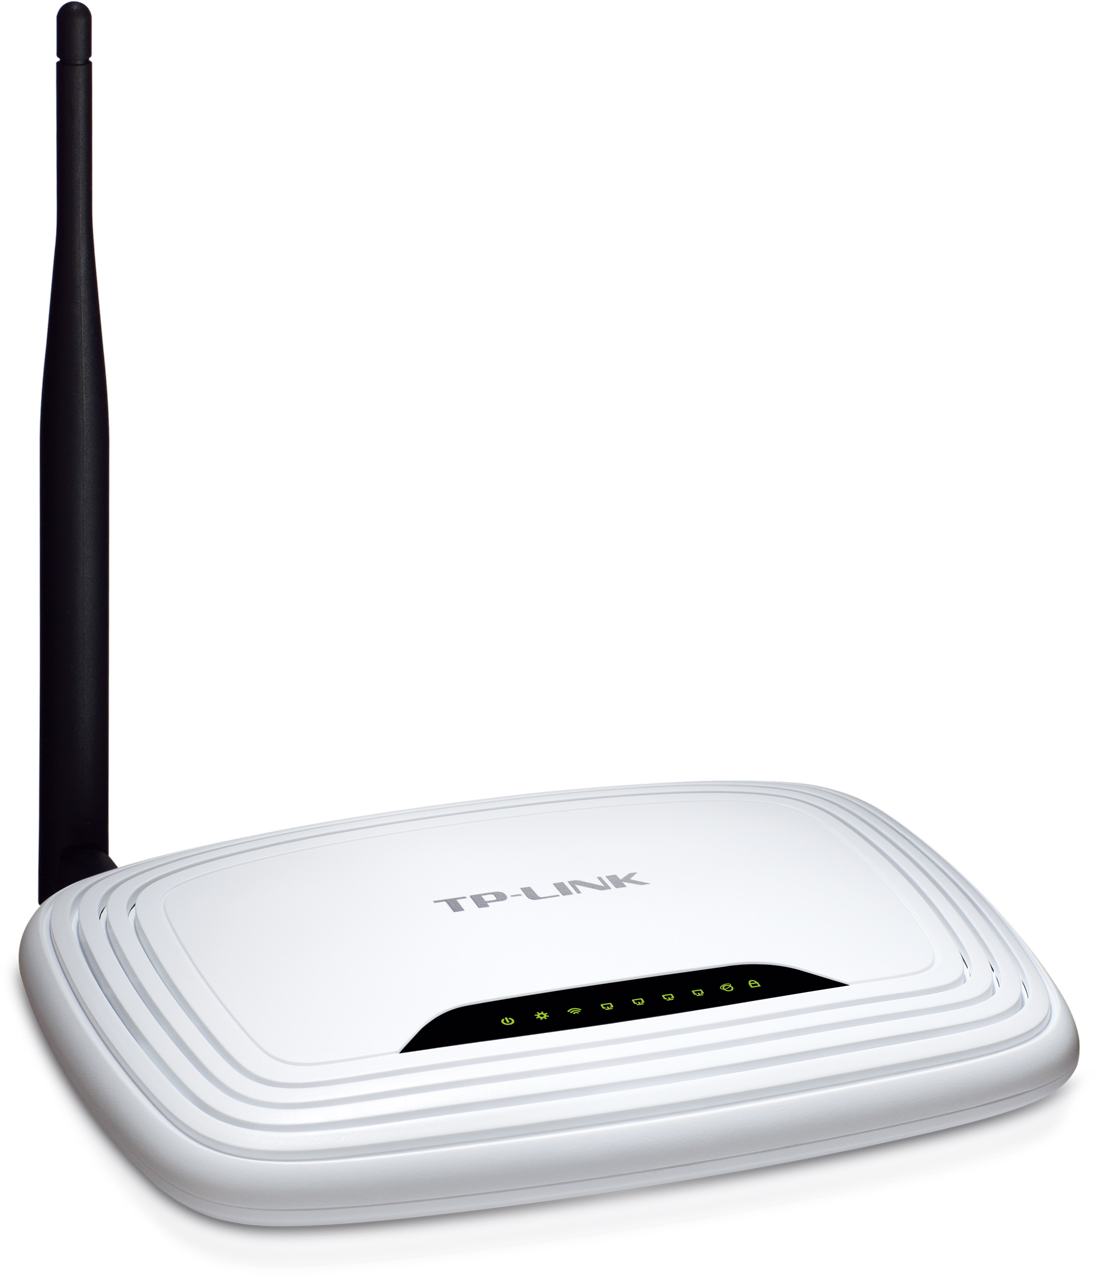
\includegraphics[width=0.26\linewidth]{Pictures/chapter4/router.jpg}
		\caption{TP-LINK TL-WR741ND}
	\end{center}
\end{figure}

To summarize, with its 150Mbps wireless data rate and its advanced WiFi security management (\texttt{WPA/WPA2} encryptions), this router provides a rather good base for our active WiFi monitoring program. But in order to be able to execute it on the probes and get results we had to change to firmware of the router to something no proprietary we can work with and we can modulate as we wish. This is why we have chosen to replace the original TP-LINK firmware installed on the router with \texttt{OpenWrt}.


\subsection{OpenWrt}
\texttt{OpenWrt}\cite{openwrt} is a highly extensible GNU/Linux distribution for embedded devices. The particularity of \texttt{OpenWrt} is that it is a full-featured, easily modifiable operation system for the routers. Indeed, it offers a fully writeable file system and a built-in package manager. Thanks to this package manager, we can install any package we want from a software repository allowing us to customize the device to suit any application. All the restrictions and configurations provided by the vendor within its own firmware installed by default on the router are therefore dropped meaning the device using this distribution can features functions such as \texttt{SSH} server, \texttt{VPN}, \texttt{BitTorrent client}, custom QoS and so on.

There are several firmwares available for \texttt{OpenWrt}. We have chosen to use the most recent one, \textit{OpenWrt 12.09 - Attitude Adjustment} for our active monitoring solution. Doing so, this ensure a reliable and up-to-date environment to deploy our application.


\subsection{Active WiFi Monitoring Solution}
Our active WiFi monitoring solution is based on a \texttt{C} program running on that \texttt{OpenWrt} router. The program uses the \texttt{wpa\_supplicant} API to be able to connect to different networks. Plus during the connection processes, a log file is created and maintained by the program to write down important information about the network's behavior. 

On this subsection we first give an overview of \texttt{wpa\_supplicant} and how we use it in our implementation. Then, we explained how our program is structured and what are the key parts that make it work and that make us able to get some insights about the networks in real time.

\subsubsection{\texttt{wpa\_supplicant}} %RSN = Robust Security Network
 As defined in \cite{wpa-supplicant}, \texttt{wpa\_supplicant} is a WPA Supplicant for Linux, BSD and Windows with support for WPA and WPA2 (\texttt{IEEE 802.11i/RSN}). Supplicant is the \texttt{IEEE 802.1X/WPA} component taht is used in the client stations. It implements key negociation with a WPA Authenticator and it can optionally control roaming and \texttt{IEEE 802.11} authentication/association of the wlan driver.

 This supplicant uses portabe \texttt{C} code and is divided into several seperate files containing independent modules besides from the core part. The core part embedded functionality for controlling the network selection, association and configuration while independent modules include code dealing with WPA (such as key handshake, pre-authentication, etc.), \texttt{EAPOL} and \texttt{EAP} state machines and methods. Also, \texttt{wpa\_supplicant} implements a control interface that we use in our program and that can control the operations of the \texttt{wpa\_supplicant} deamon.

The following figure gives an overview of all the wpa\_supplicant modules and how they interact with each other.

 \begin{figure}[H]
 	\begin{center}
		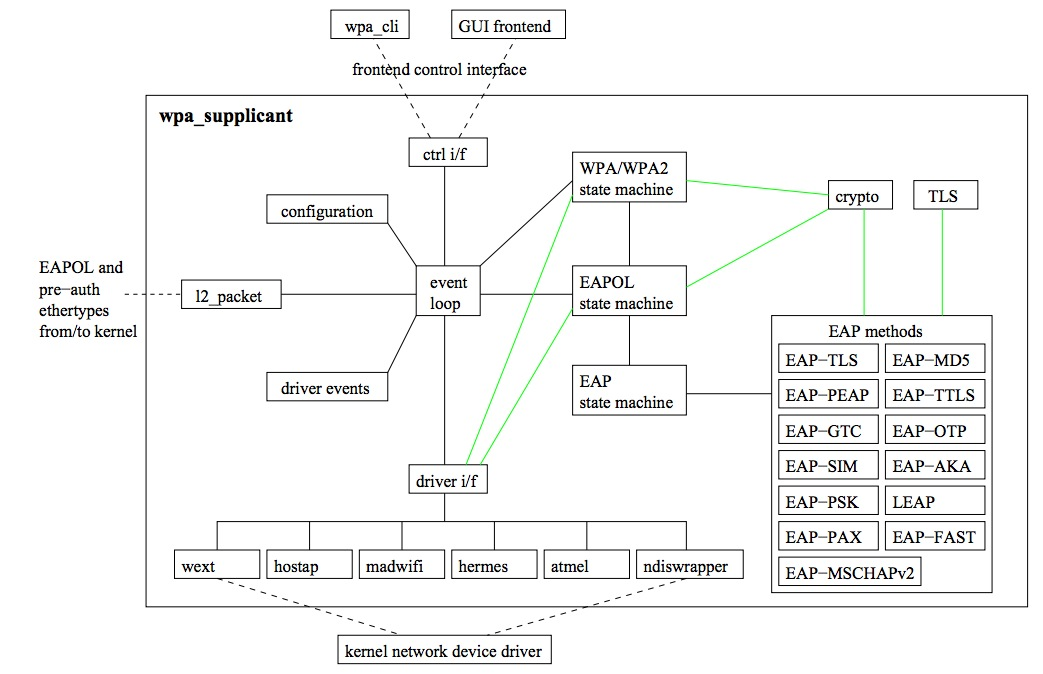
\includegraphics[width=1\linewidth]{Pictures/chapter4/wpa-supplicant-modules.jpg}
		\caption{\texttt{wpa\_supplicant} modules}
	\end{center}
\end{figure}

Within \texttt{wpa\_supplicant} there is a small \texttt{C} file, \texttt{wpa\_ctrl.c} that provides several functions to facilitate the use of that control interface. We have linked this file into program to be able to use that library of functions that can interact and communicate with \texttt{wpa\_supplicant}. Once that file is linked into the program, we can open a connection to the control interface with the \texttt{wpa\_ctrl\_open()} function and we can start sending commands to \texttt{wpa\_supplicant} with the function \texttt{wpa\_ctrl\_request()}. In order to be able to receive messages from the daemon, our program also needs to attach to the control interface using \texttt{wpa\_ctrl\_attach()}.

Several commands can be specified and sent to the \texttt{wpa\_supplicant} daemon but we only use a small selection of them, most of them being unrelated with our object of study. Here is the list of the commands used in our program and their meaning:
\begin{itemize}
	\item[-] \texttt{SCAN}: This command request the daemon to perform a new BSS scan.

	\item[-] \texttt{SCAN\_RESULTS}: This is used to get the latest scan results. Those results embed details about the bssid, the frequency, the signal level, the flags and the ssid of each network scanned. The message returned has the same syntax as in the following example representing one entry for each one of the networks of the UCL.\\

\begin{lstlisting}[frame=single,breaklines=true,caption={Scan results message exemple}]
bssid / frequency / signal level / flags / ssid
68:86:a7:30:a0:a2	2437	-56	[WPA-PSK-CCMP]	eduroam
00:1e:bd:65:34:73	2462	-55	[WPA-PSK-CCMP]	visiteurs.UCLouvain
00:1e:bd:65:34:71 	2462	-56	[WPA-PSK-CCMP]	student.UCLouvain
68:86:a7:30:a0:a0 	2437	-55	[WPA-PSK-CCMP]	UCLouvain
68:86:a7:30:a0:a4 	2437	-57	[WPA-PSK-CCMP]	UCLouvain-prive
\end{lstlisting}

	\item[-] \texttt{ADD\_NETWORK}: This commands adds a new network with empty configuration. This added network is disabled at first and can be configured afterwards. The commands returns a message containing the id of the new network or \texttt{FAIL} on failure. In our case, the program adds 5 networks at boot for the 5 networks present within the university's campus.

	\item[-] \texttt{SET\_NETWORK <network id> <variable> <value>}: Once the networks had been added with the previous command, we can configure them using this particular command. The \textit{variable} of the command uses the same variables and data formats as the standard \texttt{wpa\_supplicant} configuration file. For example, here are the different \texttt{SET\_NETWORK} commands used to configure the \texttt{student.UCLouvain} (with ID=1 for example) that we use in the program.\\

\begin{lstlisting}[frame=single,breaklines=true,caption={Configuration of the \texttt{student.UCLouvain} network}]
SET_NETWORK 1 ssid "student.UCLouvain"
SET_NETWORK 1 key_mgmt WPA-EAP
SET_NETWORK 1 eap TTLS
SET_NETWORK 1 identity "login@wifi.uclouvain.be"
SET_NETWORK 1 password "password"
SET_NETWORK 1 ca_cert "etc/wpa_supplicant/chain-radius.pem"
SET_NETWORK 1 pahse2 "auth=PAP"
\end{lstlisting}

	\item[-] \texttt{SELECT\_NETWORK <network id>}: This command asks the \texttt{wpa\_supplicant} daemon to select a special network specifying its ID. When the network is selected, all the others are disabled.

	\item[-] \texttt{DISCONNECT}: Special command to disconnect from the current network.
\end{itemize}

Thanks to does commands our program can to control the \texttt{wpa\_supplicant} daemon and is thus able to simulate a typical user's behavior connection to the networks. More information about \texttt{wpa\_supplicant} can be found inside the developer's guide\cite{wpa-supplicant-devel}.


\subsubsection{\texttt{wifi\_minitoring.c}}
In this section we describe the implementation details of our active monitoring program and how it gathers data about the current state of the networks.

The first thing the program does at boot is to start \texttt{wpa\_supplicant}. We have created an empty configuration file for the supplicant in order to launch it without starting a connection to a special network defined in that file. The supplicant uses the driver \texttt{nl80211} which is the current standard (\texttt{wext} being deprecated) and uses the \texttt{wlan0} interface.
Once the supplicant is started we open a connection with the control interface using \texttt{wpa\_ctrl\_attach(/tmp/run/wpa\_supplicant/wlan0)} (where the parameter is the path for UNIX domain sockets). That function returns a pointer to the abstract control interface data and is stored inside an internal \texttt{wpa\_ctrl} structure.






\section{Communication between Server and Probes}
The probes and the server have to exchange information. As we wanted to create a modular tool, we have chosen to encrypt all the data sent between the server and the probes. If the active monitoring device capture sensible contents, there must be no security vulnerabilities like \emph{eavesdropping} or \emph{man-in-the-middle attack}.
The first constraint that appeared was the weak computation power of the probes. In consequence, we had to keep the encryption as easy to perform as possible. So, we have looked into \emph{symmetric cryptographic} techniques. But in the other hand, as we have several probes, it could be difficult to manage and exchange the keys unlike in asymmetric cryptography. Our choice was to take the best of both worlds and implement a protocol using hybrid encryption.
In definitive, we used RSA and AES encryption together.
\subsection{RSA}
RSA\footnote{\url{http://www.google.com/patents/US4405829}} is one of the most used \emph{public-key cryptosystem}. Its name comes from its three designers: Ron Rivest, Adi Shamir, and Leonard Adleman. The algorithm involves two key: a \emph{public key} known by everybody and a \emph{private key} kept secret. The safety ensured by the technique comes from the difficulty of the factoring problem (factoring the product of two large prime numbers).
The main advantage against symmetric cryptography is that the public key used for the encryption can be known by everybody and so make the problem of key exchange a lot easier. To make the explication clearer we will present a simple example occurring between Alice and Bob.
\begin{enumerate}
\item Alice give her public key to Bob.
\item Bob wants to transmit a encrypted message to Alice. He uses the Alice's \emph{public key} to encrypt the message.
\item Bob sends his message to Alice. Even if people intercept the transmission and have the public key, they couldn't decrypt it.
\item Alice receives the message and decrypt it with her private key which she have kept secret.
\end{enumerate}
The key is 2048 bits long and each entity has its own pair of keys (i.e. the server and each probe). The server will known the authorized probes by having their private keys and will use them to encrypt the AES key (see below).
The main drawback of such encryption is that the computations are quite heavy to perform. Which is against our previous requirements. That's why we only use it to encrypt and exchange a symmetric key that will be used for the exchange of data.
\subsection{AES}
The symmetric algorithm used is AES which stands for Advanced Encryption Standard. We chose a size of 256 bits for the keys which is quite correct for our utilization. The idea is to permute the bits of the message using the key. The operations performed are lighter than the ones used by RSA and so make it more adapted to be used on the probes.

\subsection{Transaction Protocol}
To be correct, the exchanges between the probes and the server requires a protocol well defined and respected by the two parts. 



As already said, the server knows the public key of every probe in advance. 



\subsection{OpenSSL}

\subsection{PyCrypto}

\section{Deployment}
For the deployement of our system, we had a dedicated machine to host our data. This system was quite limited to be able to efficiently serve the requests. The server have a hard drive of about 300GB which is quite enough to stock the information gathered by NetwObserver during the test phase. In the other hand, the memory available was only of 1GB which is not enough to ensure a efficient handling of the users requests.

\subsection{Apache 2}
As the interface of the system is composed of Web pages, the HTTP requests are handle by Apache2. As the most used server, we had a lot of documentation available. That was the main reason of our choice. Moreover, we thought that a first experience in server configuration would be an interesting experience for any computer science students.

\subsection{Module WSGI}
This Apache module is able to interpret some python code. As said before, we choose Django as framework and in consequence executing python code is an important requirement. Something to note about the installation is that the code is written in \emph{Python3.3} and not in the version 2. That's force to be carreful during the installation as the default python interpreter in most system is the 2.6. In definitive, we have to compile the module WSGI with the specification of the right interpreter.

\subsection{Celery}
Celery\footnote{http://www.celeryproject.org/} is a distributed task queue. It allows to create asynchronous jobs handled by several workers. Concretely, a worker is a external thread that receives tasks to accomplished. the main drawback of \emph{Apache} is that it's quite complicated to generate and manage daemon running in background constantly or at given intervals. As a turn-around, we have connected our system to Celery. It helps us to manage more efficiently the concurrent elements of the application. Our server has a small memory and a poor computation power and in consequence we must manage and organise the utilization of those resources. This module has two main component: the workers and the scheduler.

\subsubsection*{The workers}
In Celery, we can define the number of workers working on the task send to the queue. By adapting this number, we can tune the allocation of the processor. For example, when we lunch a set of \emph{SNMP} requests, it can require a large part of the available resources. Each of these set of requests are lunch at different intervals and can sometime overlap. When that situation occurred, the server can experience heavy computation requirements and have trouble to handle the requests generated by the users. That's why we define a fixed number of workers and each tasks wait in a queue till a slot are available. The main drawback of such architecture is that the the precise moment when the jobs is effectively done is undetermined. Even if it can be really annoying in certain context, it is not the case in our system. Either we have a daemon that run permanently as the one handling the communication with the probes or the task have to gather some data at some interval. This last category have not precise time requirement and even if they happen dozens of minutes later, it's not a really issue here.

\subsubsection*{The Scheduler}
The scheduler in Celery is called \emph{beat} and its only responsibility is to send the \emph{periodic tasks} to the workers. We have given it the path of the application i which we have define the task and the related interval. \emph{Celery beat} gatherer them and fire the task accordingly. The main warning about the scheduler is the fact that it lunch the task \textbf{exactly} at each interval. If we imagine a task that take between 4 and 5 minutes to be perform and that the interval is of 10 minutes, there can be moments where two instances of that tasks overlap. Effectively, if all the workers are occupied and the first instance only start after 8 minutes of waiting, the second task will start two minutes later while the first one is still running. Here again, such consideration have been taken care of and the data are store with a time stamp or linked to en entity having one. The data gatherer can be completely order and even if such condition occurred, the result would be only a lack of data during an interval and more during the next one. As the intervals vary from 20 minutes to 2 hours while the results are analyse throught several day of data, the impact is quite reduced. 

\section{Extensions and Portability}
